\documentclass{article}
\usepackage[utf8]{inputenc}
\usepackage{amsmath, amssymb, amsthm}
\usepackage{float}

\usepackage{listings}
\usepackage{xcolor}

\usepackage{tikz}
\usepackage{float}

\newtheorem{theorem}{Theorem}[section]

% \theoremstyle{definition}

% \newtheorem{rules}{Rule}[section]
% \newtheorem{definition}[rules]{Definition}
% \newtheorem{remark}[rules]{Remark}
% \newtheorem{example}[rules]{Example}

\definecolor{codegreen}{rgb}{0,0.6,0}
\definecolor{codegray}{rgb}{0.5,0.5,0.5}
\definecolor{codepurple}{rgb}{0.58,0,0.82}
\definecolor{backcolour}{rgb}{0.95,0.95,0.92}

\lstdefinestyle{thestyle}{
    backgroundcolor=\color{backcolour},
    basicstyle=\ttfamily\footnotesize,
    keywordstyle=\color{red!80}\bfseries,
    ndkeywordstyle=\color{blue!80}\bfseries,
    identifierstyle=\color{black},
    commentstyle=\color{codegreen},
    stringstyle=\color{codepurple},
    breakatwhitespace=false,
    breaklines=true,
    captionpos=b,
    keepspaces=true,
    numberstyle=\tiny\color{codegray},
    numbers=left,
    numbersep=2pt,
    showspaces=false,
    showstringspaces=false,
    showtabs=false,          
    tabsize=2
}

\lstset{style=thestyle}

\lstdefinelanguage{TML}{ 
    keywords={changeto, move, goto, if, while, module, accept, reject, halt, alphabet},
    ndkeywords={left, right, blank},
    sensitive=true,
    comment=[l]{//},
    morecomment=[s]{/*}{*/},
    morestring=[b]',
    morestring=[b]"
}

\usetikzlibrary{automata}

\title{Proof of Equivalence}
\author{Pete Gautam}

\begin{document}
    \maketitle

    In this document, we give a proof of equivalence between TMs and TML programs. This is done in many steps that involve:
    \begin{itemize}
        \item proving that a TM can be converted to a complete TML program;
        \item proving that a complete TML program can be converted to a TM; and
        \item proving that a valid TML program can be converted to a complete TML program.
    \end{itemize}

    \section{Complete TML Programs}
    When we defined execution of a valid TML program on a tape in the specification, we said that a basic block need not have all 3 types of commands (\textit{changeto}, \textit{move} and a \textit{flow} command), but in the execution above, we have established some `default' ways in which a program gets executed. In particular,
    \begin{itemize}
        \item if the \textit{changeto} command is missing, we do not change the value of the tape;
        \item if the \textit{move} command is missing, we move left;
        \item if the \textit{flow} command is missing, we can establish what to do using the rules described above- this is a bit more complicated than the two commands above.
    \end{itemize}
    Nonetheless, it is possible to include these `default' commands to give a \emph{complete} version of the program. This is what we will establish in this section. 

    Consider the following complete program.
\begin{lstlisting}[language=TML]
alphabet = {0, 1}
module isOdd {
    // move to the end
    while 0 {
        changeto 0
        move right
    } while 1 {
        changeto 1
        move right
    } if blank {
        changeto blank
        move left
        goto isOddCheck
    }
}
module isOddCheck {
    // accept if and only if the value is 1
    if 0, blank {
        changeto 0
        move left
        reject
    } if 1 {
        changeto blank
        move left
        accept
    }
}
\end{lstlisting}
    Now, we consider the rules that a complete TML program obeys:
    \begin{itemize}
        \item A basic block in a complete program has all the necessary commands- if the basic block is inside \textit{while} case, it has a \textit{changeto} command and a \textit{move} command; otherwise, it also has a \textit{flow} command.
        \item A module in a complete program is composed of a single switch block.
    \end{itemize}

    We will now construct a complete TML program for a valid TML program.
    \begin{enumerate}
        \item We first break each module into smaller modules so that every module has just one basic/switch block- we add a \textit{goto} command to the next module if it appeared just below this block.
        \item Then, we can convert each basic block to a switch block by just adding a single case that applies to each letter in the alphabet.
        \item Finally, we add the default values to each basic block to get a complete TML program.
    \end{enumerate}
    This way, we can associate every block in the valid program with a corresponding block in the complete program. The complete version is always a switch block and might have more commands than the original block, but it still has all the commands present in the original block. 

    We now illustrate this process with an example. Assume we first have the following program.
\begin{lstlisting}[language=TML]
alphabet = {a, b}
module simpleProgram {
    changeto b
    move left
    move right
    accept
}
\end{lstlisting}
    In step 1 of the completion process, we create a module for each block. In this program, there are two basic blocks- at lines 3-4 and 5-6. So, after applying the first step, we get the following program.
\begin{lstlisting}[language=TML]
alphabet = {a, b}
module simple1 {
    changeto b
    move left
    goto simple2
}
module simple2 {
    move right
    accept
}
\end{lstlisting}
    In this case, we have two basic blocks at lines 3-5 and 8-9. So, in step 2, we convert them into switch blocks and get the following program.
\begin{lstlisting}[language=TML]
alphabet = {a, b}
module simple1 {
    if a, b, blank {
        changeto b
        move left
        goto simple2
    }
}
module simple2 {
    if a, b, blank {
        move right
        accept
    }
}
\end{lstlisting}
    Finally, we add all the default values in step 3 and get the following program.
\begin{lstlisting}[language=TML]
alphabet = {a, b}
module simple1 {
    if a {
        changeto b
        move left
        goto simple2
    } if b {
        changeto b
        move left
        goto simple2
    } if blank {
        changeto b
        move left
        goto simple2
    }
}
module simple2 {
    if a {
        changeto a
        move right
        accept
    } if b {
        changeto b
        move right
        accept
    } if blank {
        move right
        accept
    }
}
\end{lstlisting}
    This program obeys the definition of a complete program.

    \begin{theorem} \label{thm:complete_TM}
        Let $P$ be a valid TML program. Then, $P$ and its completion $P^+$ execute on every tape $T$ in the same way. That is,
        \begin{itemize}
            \item for every valid index $n$, if we have tape $T_n$, tapehead index $i_n$ and module $m_n$ with executing block $b_n$ for the TML program $P$, and we have tape $S_n$, tapehead index $j_n$ and module $t_n$, then $T_n = S_n$, $i_n = j_n$, and $t_n$ is the corresponding complete module block of $b_n$;
            \item $P$ terminates execution on $T$ if and only if $P^+$ terminates execution on $T$, with the same final status (\texttt{accept} or \texttt{reject}).
        \end{itemize}
    \end{theorem}
    \begin{proof}
        We prove this by induction on the execution step (of the tape). 
        \begin{itemize}
            \item At the start, we have the same tape $T$ for both $P$ and $P^+$, with tapehead index 0. Moreover, the corresponding (completed) module of the first block in the first module of $P$ is the first module of $P$. So, the result is true if $n = 0$. 
            \item Now, assume that the result is true for some integer $n$, where the block $b_n$ in the TML program $P$ does not end with a terminating \textit{flow} command. Let $\sigma_n$ be the letter at index $i_n = j_n$ on the tape $S_n = T_n$.
            \begin{itemize}
                \item If the \textit{changeto} command is missing in $b_n$ for $\sigma_n$, then the next tape $T_{n+1} = T_n$. In the complete module $m_n$, the case for $\sigma_n$ will have the command \texttt{changeto} $\sigma_n$. So, the next tape is given by:
                \[S_{n+1}(x) = \begin{cases}
                    S_n(x) & x \neq j_n \\
                    \sigma_n & \text{otherwise}
                \end{cases}.\]
                Therefore, we have $S_{n+1} = S_n$ as well. So, $T_{n+1} = S_{n+1}$. Otherwise, we have the same \textit{changeto} command in the two blocks, in which case $T_{n+1} = S_{n+1}$ as well.
                
                \item If the \textit{move} command is missing in $b_n$ for $\sigma_n$, then the next tapehead index $i_{n+1} = i_n - 1$. In the complete module $m_n$, the case for $\sigma_n$ will have the command \texttt{move left}, so we also have $j_{n+1} = j_n - 1$. Applying the inductive hypothesis, we have $i_{n+1} = j_{n+1}$. Otherwise, we have the same \textit{move} command, meaning that $i_{n+1} = j_{n+1}$ as well.
                
                \item We now consider the next block $b_{n+1}$:
                \begin{itemize}
                    \item If the block $b_n$ is a \textit{switch} block with a \textit{while} case for $\sigma_n$, then this is still true in the module $m_n$. So, the next block to be executed in $P$ is $b_n$, and the next module to be executed in $P^+$ is $m_n$. In that case, the corresponding module of the block $b_{n+1} = b_n$ is still $m_{n+1} = m_n$.
        
                    \item Instead, if the block $b_n$ has no \textit{flow} command for $\sigma_n$, and is not the last block, then the next block to execute is the block just below $b_n$, referred as $b_{n+1}$. By the definition of $P^+$, we find that the case block in the module $m_n$ has a \textit{goto} command, going to the module $m_{n+1}$ which corresponds to the block $b_{n+1}$. 
                
                    \item Now, if the \textit{flow} command is missing for $\sigma_n$ and this is the last block, then execution is terminated with the status \texttt{reject} for the program $P$. In that case, the case for $\sigma_n$ in the module $m_n$ has the \texttt{reject} command present, so the same happens for $P^+$ as well. 
                
                    \item Otherwise, both $P$ and $P^+$ have the same flow command, meaning that there is either correspondence between the next module to be executed, or both the program terminate with the same status. 
                \end{itemize}
            \end{itemize}
        \end{itemize}
        In that case, $P$ and $P^+$ execute on $T$ the same way by induction.
    \end{proof}

    \section{Equivalence of TMs and TMLs}
    In this section, we will show that there is an equivalence between TMs and valid TML programs. We will first construct a valid TML program for a TM and then show that it has the same behaviour as the TM. Later, we will construct a TM for a TML program, and show the equivalence in this case as well.

    \begin{figure}[htb]
        \centering
        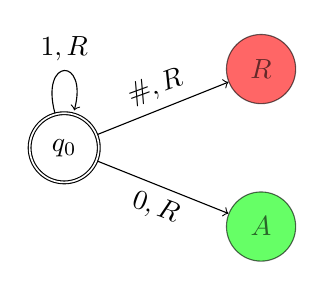
\begin{tikzpicture}
            \node[state, accepting] (q1) at (2.5, 0) {$q_0$};
            \node[state, fill=green, opacity=0.6] (A) at (5, -1) {$A$};
            \node[state, fill=red, opacity=0.6] (R) at (5, 1) {$R$};

            \draw[->] (q1) edge[loop above] node[above] {$1, R$} (q1);
            \draw[->] (q1) -- node[below, rotate=-20] {$0, R$} (A);
            \draw[->] (q1) -- node[above, rotate=20] {$\#, R$} (R);
        \end{tikzpicture}
        \caption{A TM that accepts binary strings containing 0}
        \label{fig:simple_tm}
    \end{figure}
    We will first illustrate how to convert a TM to a (complete) TML program. So, consider the TM at Figure \ref{fig:simple_tm}. Then, its corresponding TML program is the following:
\begin{lstlisting}[language=TML]
alphabet = {0, 1}
module has0 {
    if 1 {
        changeto 1
        move right
        goto has0
    } if 0 {
        changeto 0
        move right
        accept
    } if blank {
        changeto blank
        move left
        reject
    }
}
\end{lstlisting}
    In general, we convert each (non-terminating) state in the TM $M$ to a TML module. The following is how we create the module:
    \begin{itemize}
        \item the module contains a single \textit{switch} command;
        \item for each letter $\sigma$ in the alphabet $\Sigma^+$, denote $\delta(q, \sigma) = (q', \sigma', \texttt{dir})$. We add an \textit{if} case in the \textit{switch} command corresponding to letter $\sigma$ with the following commands:
        \begin{itemize}
            \item \texttt{changeto} $\sigma'$
            \item \texttt{move} \textit{dir}
            \item if $q'$ is \texttt{accept}, then the command \texttt{accept}; if $q'$ is \texttt{reject}, then the command \texttt{reject}; otherwise, \texttt{goto} $q'$.
        \end{itemize}
    \end{itemize}
    Moreover, we can construct the program $P$ with:
    \begin{itemize}
        \item the alphabet $\Sigma$;
        \item modules corresponding to every state $q$ in $M$;
        \item the module corresponding to the initial state $q_0$ placed at the top.
    \end{itemize}
    We say that $P$ is the \emph{corresponding program for $M$}.

    \begin{theorem} \label{thm:TM_to_TMP}
        Let $M$ be a TM, and let $P$ be the corresponding program for $M$. Then, $M$ and $P$ execute on every tape $T$ in the same way. That is, 
        \begin{itemize}
            \item for every valid index $n$, if we have tape $T_n$, tapehead index $i_n$ and module $m_n$ for the TML program $P$, and we have tape $S_n$, tapehead index $j_n$ and state $q_n$ for the TM $M$, then $T_n = S_n$, $i_n = j_n$ and $m_n$ is the corresponding module for $q_n$;
            \item $M$ terminates execution on $T$ if and only if $P$ terminates execution on $T$, with the same final status (\texttt{accept} or \texttt{reject}).
        \end{itemize}
    \end{theorem}
    \begin{proof}
        We prove this by induction on the execution step. 
        \begin{itemize}
            \item At the start, we have the same tape $T$ for both $M$ and $P$, with tapehead index $0$. Moreover, the first module in $P$ corresponds to the initial state $q_0$. So, the result is true if $n = 0$.
            
            \item Now, assume that the result is true for some integer $n$, where the TM state $q_n$ is not \texttt{accept} or \texttt{reject}. In that case, $T_n = S_n$, $i_n = j_n$ and $m_n$ is the corresponding module for $q_n$. Let $\sigma_n$ be the letter at index $i_n = j_n$ on the tape $T_n = S_n$. Denote $q(q_n, \sigma_n) = (q_{n+1}, \sigma_{n+1}, \texttt{dir})$. In that case,
            \[T_{n+1}(x) = \begin{cases}
                T_n(x) & x \neq i_n \\
                \sigma_{n+1} & \text{otherwise},
            \end{cases} \qquad i_{n+1} = \begin{cases}
                i_n - 1 & \texttt{dir} = \texttt{left} \\
                i_n + 1 & \texttt{dir} = \texttt{right},
            \end{cases}\]
            and the next state is $q_{n+1}$. 
            
            \begin{itemize}
                \item We know that the module $m_n$ in TML program $P$ corresponds to the state $q_n$, so it has a \texttt{changeto} $\sigma_{n+1}$ command for the case $\sigma_n$. In the case, the next tape for $P$ is:
                \[S_{n+1}(x) = \begin{cases}
                    S_n(x) & x \neq i_n \\
                    \sigma_{n+1} & \text{otherwise}.
                \end{cases}\]
                So, $T_{n+1} = S_{n+1}$. 
                
                \item Similarly, the case also contains a \texttt{move dir} command. This implies that the next tapehead index for $P$ is:
                \[j_{n+1} = \begin{cases}
                    j_n - 1 & \texttt{dir} = \texttt{left} \\
                    j_n + 1 & \texttt{dir} = \texttt{right}.
                \end{cases}\]
                Hence, $i_{n+1} = j_{n+1}$. 
            
                \item Next, we consider the value of $q_{n+1}$:
                \begin{itemize}
                    \item If $q_{n+1} = q_n$, then the case block is a \textit{while} block, and vice versa. So, the next module to be executed is $m_n$. In that case, $m_{n+1}$ still corresponds to $q_{n+1}$.
                    \item Otherwise, we have an \textit{if} block. 
                    \begin{itemize}
                        \item In particular, if $q_{n+1}$ is the \texttt{accept} state, then the case for $\sigma_n$ contains the \textit{flow} command \texttt{accept}, and vice versa. In that case, execution terminates with the same final status of \texttt{accept}. The same is true for \texttt{reject}. 
                        \item Otherwise, the module contains the command \texttt{goto} $m_{n+1}$, where $m_{n+1}$ is the corresponding module for $q_{n+1}$.
                    \end{itemize}
                \end{itemize}
            \end{itemize}
        \end{itemize}
        In that case, $P$ and $M$ execute on $T$ the same way by induction.
    \end{proof}

    Next, we construct a TM for a TML program. This process is essentially the inverse of the one we saw converting a TML program to a TM. In particular, for each module $m$ in $P$, we construct the state $q$ as follows- for each letter $\sigma$ in $\Sigma^+$, we define $\delta(q, \sigma) = (q', \sigma', \texttt{dir})$, where:
    \begin{itemize}
        \item the value $\sigma'$ is the letter given in the \textit{changeto} command within $m$;
        \item the value \texttt{dir} is the direction given in the \textit{move} command within $m$;
        \item if the \textit{flow} command in $m$ corresponding to $\sigma$ is \texttt{accept}, then $q'$ is the \texttt{accept} state; if it is \texttt{reject}, then $q'$ is the \texttt{reject} state; if we are in a \textit{while} block, then $q' = q$; otherwise, $q'$ is the state corresponding to the module given in the \textit{goto} command.
    \end{itemize}
    Then, the TM with all the states $q$, the same alphabet $\Sigma$, the transition function $\delta$ and initial state $q_0$ corresponding to the first module in $P$ is the \emph{corresponding TM for $P$}. 

    \begin{figure}[htb]
        \centering
        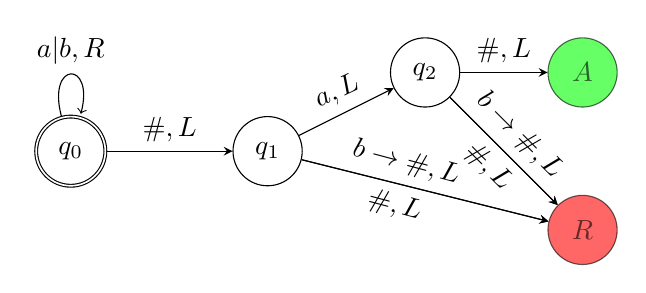
\begin{tikzpicture}
            \node[state, accepting] (s0) at (-0.5, 0) {$q_0$};
            \node[state] (s1) at (2, 0) {$q_1$};
            \node[state] (s2) at (4, 1) {$q_2$};
            \node[state, fill=green, opacity=0.6] (A) at (6, 1) {$A$};
            \node[state, fill=red, opacity=0.6] (R) at (6, -1) {$R$};
            
            \draw[-stealth] (s0) edge[loop above] node {$a|b, R$} (s0);
            \draw[-stealth] (s0) -- node[above] {$\#, L$} (s1);

            \draw[-stealth] (s1) -- node[above, rotate=25] {$a, L$} (s2);
            \draw[-stealth] (s1) -- node[below, rotate=-15, pos=0.4] {$\#, L$} (R);
            \draw[-stealth] (s1) -- node[above, rotate=-15, pos=0.4] {$b \to \#, L$} (R);

            \draw[-stealth] (s2) -- node[above] {$\#, L$} (A);

            \draw[-stealth] (s2) -- node[above, rotate=-45] {$b \to \#, L$} (R);
            \draw[-stealth] (s2) -- node[below, rotate=-45] {$\#, L$} (R);
        \end{tikzpicture}
        \caption{The TM corresponding to the program above. The state $q_0$ corresponds to the module \texttt{moveToEnd}; the state $q_1$ corresponds to the module \texttt{checkAFirst}; and the state $q_2$ corresponds to the module \texttt{checkASecond}.}
        \label{fig:tm_from_tml}
    \end{figure}

    We now illustrate this process with an example. So, consider the following TML program:
\begin{lstlisting}[language=TML]
alphabet = {a, b}
module moveToEnd {
    while a {
        changeto a
        move right
    } while b {
        changeto b
        move right
    } if blank {
        changeto blank
        move left
        goto checkAFirst
    }
}
module checkAFirst {
    if a {
        changeto blank
        move left
        goto checkASecond
    } if b, blank {
        changeto blank
        move left
        reject
    }
}
module checkASecond {
    if a {
        changeto blank
        move left
        accept
    } if b, blank {
        changeto blank
        move left
        reject
    }
}
\end{lstlisting}
    Then, its corresponding TM is given in Figure \ref{fig:tm_from_tml}.
    \begin{theorem}
        Let $P$ be a TML program, and let $M$ be the corresponding TM for $P$. Then, $P$ and $M$ execute on every tape $T$ in the same way. That is,
        \begin{itemize}
            \item for every valid index $n$, if we have tape $T_n$, tapehead index $i_n$ and module $m_n$ for TML program $P$, and we have tape $S_n$, tapehead index $j_n$ and state $q_n$ for the TM $M$, then $T_n = S_n$, $i_n = j_n$ and $q_n$ is the corresponding state for $m_n$;
            \item $P$ terminates execution on $T$ if and only if $M$ terminates execution on $T$, with the same final status (\texttt{accept} or \texttt{reject}).
        \end{itemize}
    \end{theorem}
    \begin{proof}
        Without loss of generality, assume that $P$ is complete. We prove this as well by induction on the execution step of the tape. 
        \begin{itemize}
            \item At the start, we have the same tape $T$ for both $P$ and $M$, with tapehead index $0$. Moreover, the initial state $q_0$ in $M$ corresponds to the first module in $P$. So, the result is true if $n = 0$. 
            
            \item Now, assume that the result is true for some integer $n$, which is not the terminating step in execution. In that case, $S_n = T_n$, $j_n = i_n$ and $q_n$ is the corresponding state for $m_n$. Let $\sigma_n$ be the letter at index $j_n = i_n$ on the tape $S_n = T_n$. We now consider the single switch block in $m_n$:
            \begin{itemize}
                \item If the block in $m_n$ corresponding to $\sigma_n$ is a \textit{while} block, then we know that its body is partially complete, and so is composed of the following commands:
                \begin{itemize}
                    \item \texttt{changeto} $\sigma_{n+1}$
                    \item \texttt{move dir}
                \end{itemize}
                So, we have $\delta(q_n, \sigma_n) = (q_n, \sigma_{n+1}, \texttt{dir})$. Using the same argument as in Theorem \ref{thm:TM_to_TMP}, we find that $T_{n+1} = S_{n+1}$ and $i_{n+1} = j_{n+1}$. Also, $q_{n+1} = q_n$ is the corresponding state for $m_{n+1} = m_n$. 
                
                \item Otherwise, we have an \textit{if} command. In this case, the case body is complete, and so composed of the following commands:
                \begin{itemize}
                    \item \texttt{changeto} $\sigma_{n+1}$
                    \item \texttt{move dir}
                    \item \texttt{accept}, \texttt{reject} or \texttt{goto} $m_{n+1}$.
                \end{itemize}
                So, we have $\delta(q_n, \sigma_n) = (q_{n+1}, \sigma_{n+1}, \texttt{dir})$, where $q_{n+1}$ is the corresponding state to the \textit{flow} command present. Here too, we have $T_{n+1} = S_{n+1}$ and $i_{n+1} = j_{n+1}$ by construction. 
            \end{itemize}
            Now, we consider the flow command:
            \begin{itemize}
                \item If we have an \texttt{accept} command in the body, then $q_{n+1}$ is the accepting state, and vice versa. So, we terminate execution with the final status of \texttt{accept}. The same is true for \texttt{reject}. 
                \item Otherwise, the state $q_{n+1}$ is the corresponding state to the module $m_{n+1}$.
            \end{itemize}
            In all cases, there is a correspondence between the state for $m_{n+1}$ and $q_{n+1}$.   
        \end{itemize}
        So, the result follows from induction.
    \end{proof}

    Hence, we have established that for any valid TML program, there is a TM, and vice versa.

    \section{TML as a model of computation}
    Since TML programs and TMs are equivalent, this implies that TML programs are a model for computation. Note that while we have given a proof for equivalence for TMs, this representation is based on accepting and rejecting programs only. Not all TMs are of this form. In particular, it is also possible for a TM to halt instead of accepting or rejecting.

    Although the equivalence is limited to a subclass of TMs, we can add another flow command \texttt{halt} that mimics the halting behaviour. However, this is not necessary- we can use the accept state (or equally the reject state) to mimic the behaviour of halting. Since accepting or rejecting results in the program halting, we can simply disregard the final result, and possibly read the output from the tape to infer the actual result.
\end{document}